\documentclass[a4paper,11pt]{article}
\usepackage[top=2.5cm,bottom=3cm,right=3cm,left=3cm]{geometry}
\usepackage[utf8]{inputenc}
\usepackage[T1]{fontenc}
\usepackage[french]{babel}
\usepackage{graphicx,graphics,textcomp,setspace,lettrine}
\usepackage{amsmath,amssymb,amsfonts,indentfirst}
\usepackage[toc,page]{appendix} 
\usepackage{float}
\usepackage{array}
\usepackage{comment}
\usepackage{xcolor}
\usepackage{listings}
\usepackage{blindtext}
\usepackage{titling}
\usepackage{multicol}

\usepackage[english, status=draft]{fixme}
\fxusetheme{color}

\lstset{numbers=left,
numberstyle=\tiny \bf ,
stepnumber=1,
numbersep=10pt,
firstnumber=1,
numberfirstline=true}

\lstset{frame=TBlr,
rulesepcolor=\color{black}}

\DeclareMathOperator{\e}{e}

\usepackage{fancyhdr}
\pagestyle{fancy}

\renewcommand{\headrulewidth}{1pt}
\fancyhead[L]{\leftmark}
\fancyhead[R]{}

\renewcommand{\footrulewidth}{1pt}
\fancyfoot[C]{\textbf{\thepage}} 
\fancyfoot[L]{}

\graphicspath{{results/}}

\title{{\textsc{\Large{Rapport de Méthodologie}\\ [3cm]
      \textbf{\LARGE{Amas de galaxies \\ de Planck}} \\ [0.6cm] 
Etude à travers l'effet \\ Sunyaev-Zel’dovich}} \\[2cm]}
\vfill
\author{Geoffroy de la Vieuville \\ Antoine Marchal}
\date{}


\begin{document}
\begin{titlingpage}
\maketitle
\begin{abstract}
  La collaboration Planck a extrait sur l'ensemble de la mission un
  catalogue d'amas de galaxie (PSZ2) basé sur la détection de l'effect
  Sunyaev-Zel’dovich (SZ). Nous avons, à l'aide de celui-ci,
  reconstruit par ILC (Internal Linear Combination) des estimateurs du
  CMB et de l'effet SZ thermique pour chaque amas. 
  L'étude des poids $w(\nu)$ donnés aux six fréquences des 
  maps de Planck nous apportent une vision sur les différents
  phénomènes physiques pouvant intervenir dans l'extraction de ces données. Enfin,
  l'application d'une photométrie d'ouverture nous a ensuite permis 
  d'étudier quelques propriétés de ces amas comme le flux $F=f(z)$ 
  ou encore le rayon critique photométrique $R_{c}=f(z)$.
\end{abstract}
\end{titlingpage}
%\tableofcontents
%\thispagestyle{empty}

\newpage

\section{L'effet Sunyaev-Zel’dovich}

\begin{figure}[b!]
  \centering
  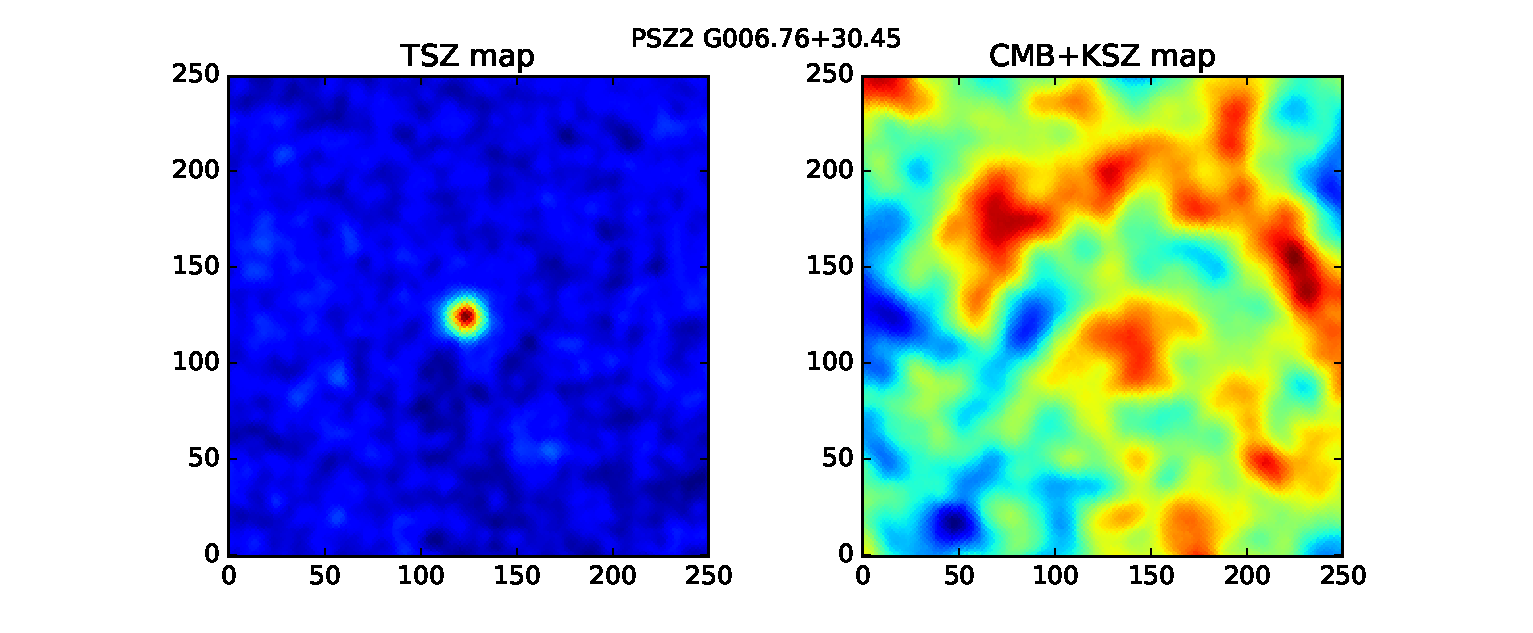
\includegraphics[width=4.5in]{sz_effect.eps}
  \label{sz_effect}
  \caption{Séparation par méthode ILC de la composante TSZ (gauche) et de la
    composante CMB+KSZ (droite) pour l'amas G006.76+30.45 du catalogue
  PSZ2}
\end{figure}

L'effet Sunyaev-Zel’dovich \cite{Sunyaev} est provoqué par la diffusion Compton
Inverse des photons du CMB par le gaz d'électrons chauds ($k_B T_e
\lesssim 15$ KeV) présent dans les amas de galaxies. Son application à
la cosmologie est capitale puisqu'il est, de part sa nature, 
théoriquement indépendant du redshift. Il permet donc l'étude de la
distribution des amas qui est un des enjeux important dans la
compréhension du modèle standard de la cosmologie et notamment de la
formation des grandes structures. Son équation est donnée par : 

\begin{align*}
  \frac{\Delta T_{SZE}}{T_{CMB}} = f(\nu) \times  y
\end{align*}

\begin{align*}
  y = \int_{l.o.s} \frac{kT_e}{m_e c^2} n_e \sigma_T dl 
\end{align*}
où $k$ is est la constante Boltzmann, $m_e$ la masse des electrons, $c$
la vitesse de la lumière, $\sigma_T$ la section efficace de Thomson, 
$n_e$ la densité d'electrons et $T_e$ la température des electrons.

\begin{align*}
  f(\nu) = x(\nu) \frac{\e^{x(\nu)}+1}{\e^{x(\nu)}-1} - 4
\end{align*}

\begin{align*}
  x(\nu) = \frac{h \nu}{k T_{CMB}}
\end{align*}

Deux composantes sont à distinguer, l'effet SZ thermique (TSZ)
explicité ci-dessus, et l'effet SZ cinétique (KSZ). La deuxième composante est simplement dù à un effet
Doppler additionnel. 

\section{Application de la méthode ILC}

\begin{figure}[b!]
  \centering
  \label{w_lat}
  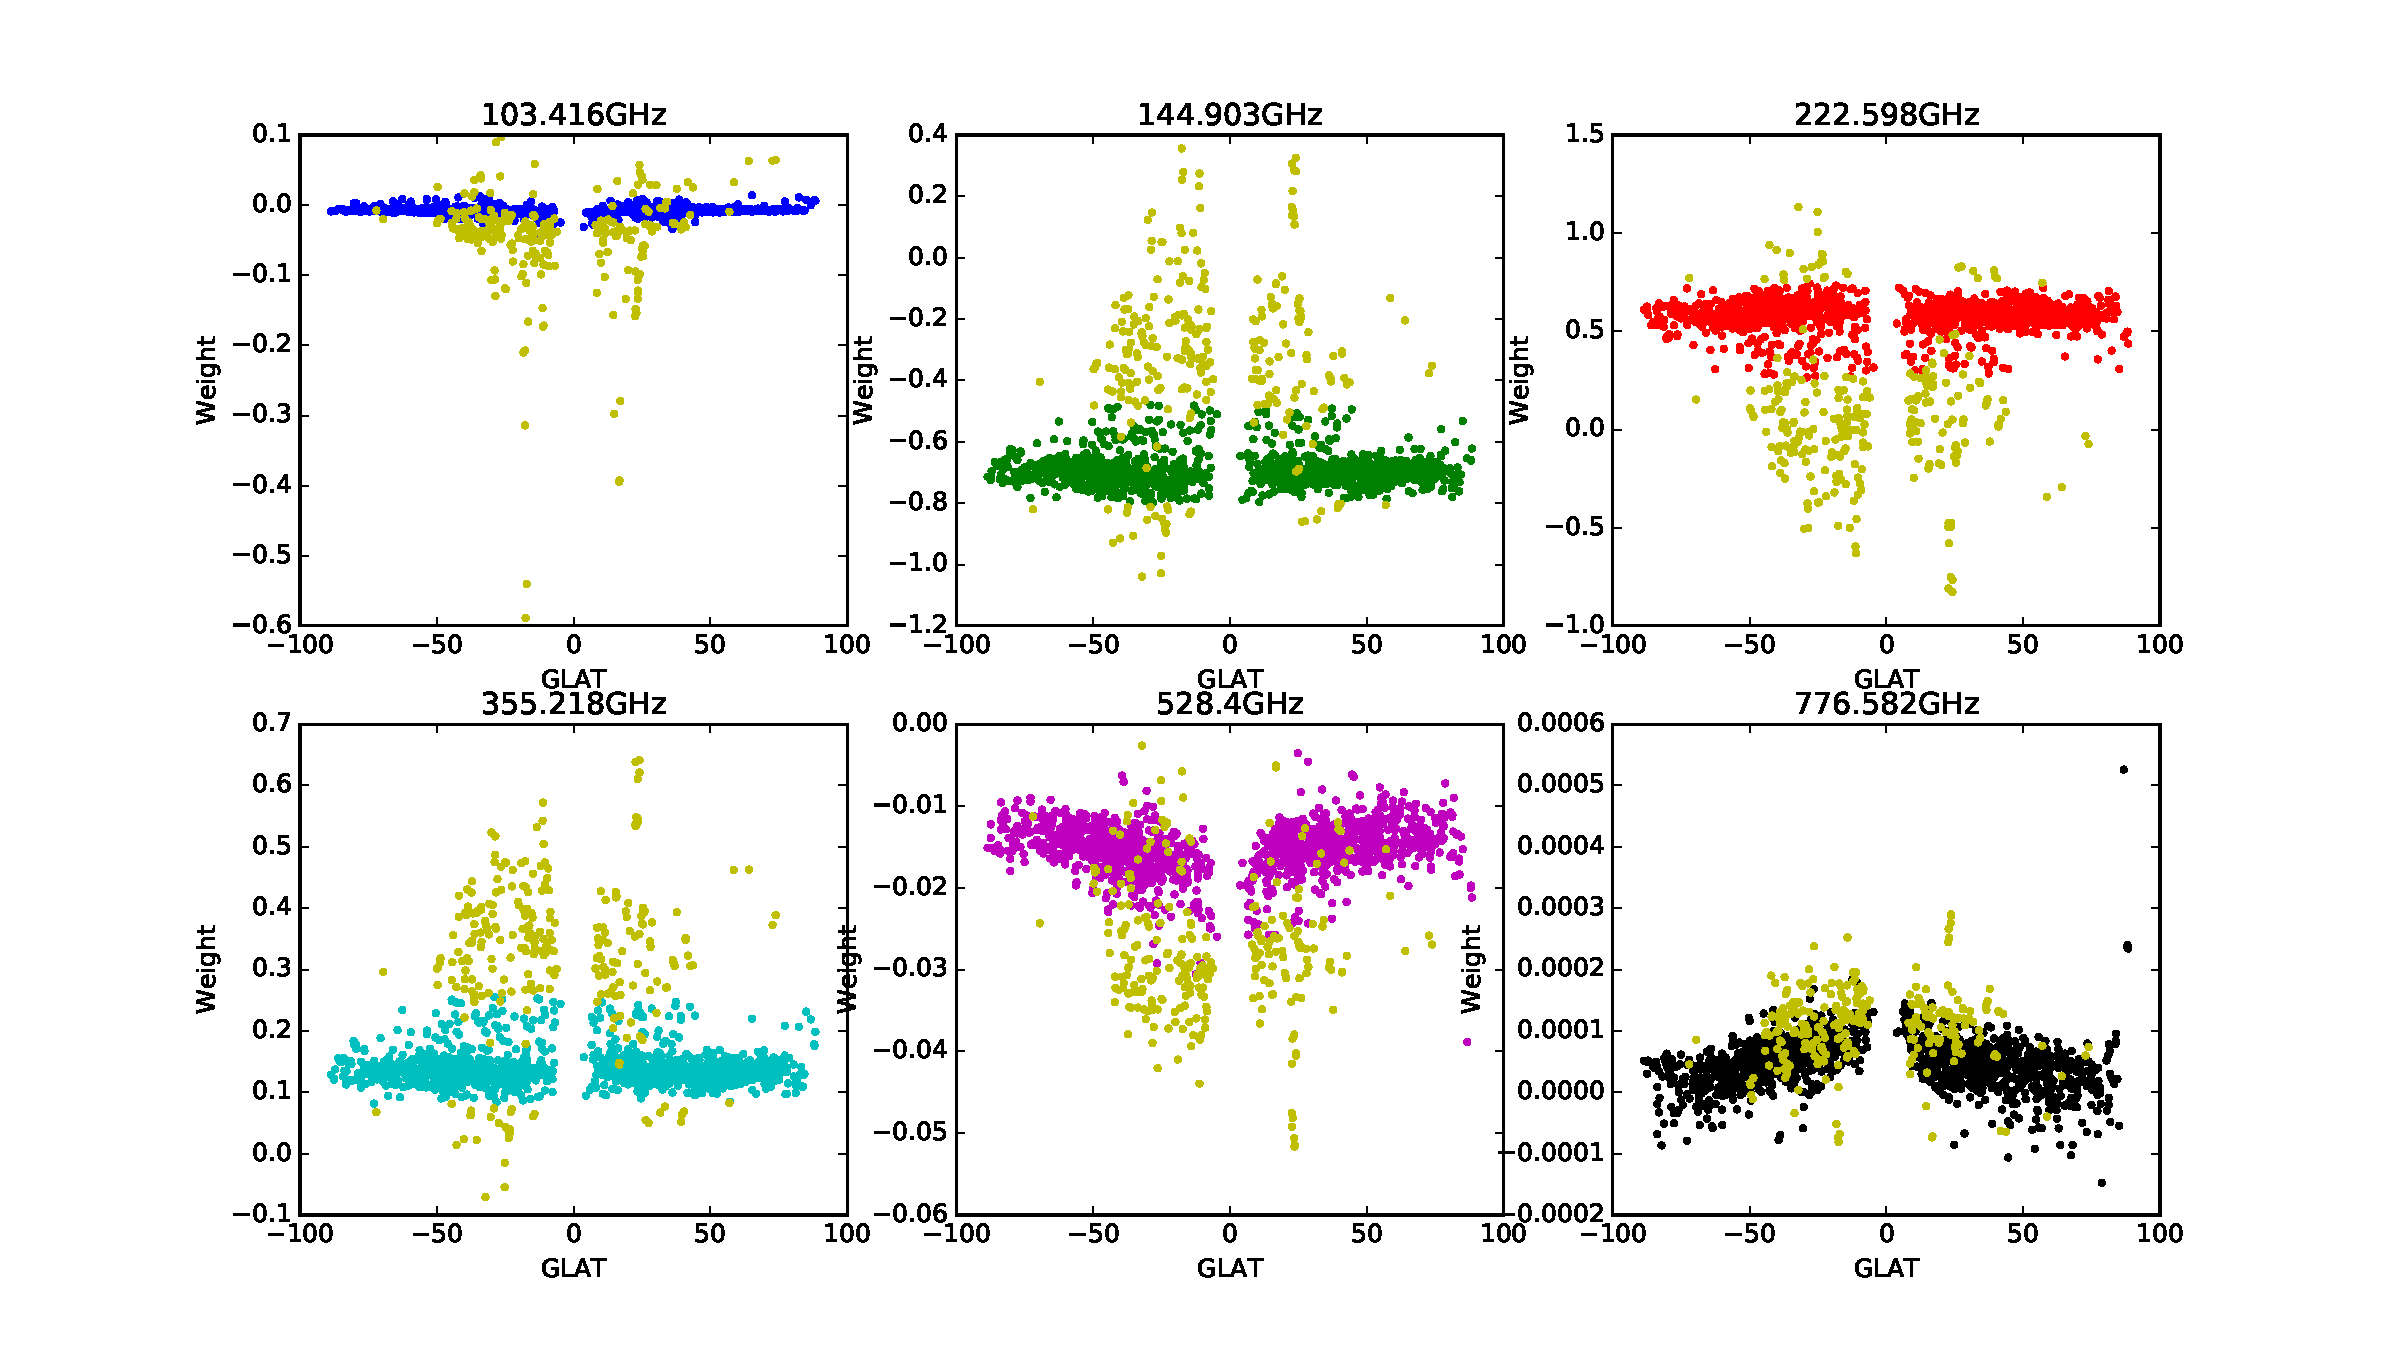
\includegraphics[width=6in]{w_lat.pdf}
  \caption{Etude des poids appliqués à chacune des six fréquences en
    fonction de la latitude en coordonnée galactique pour
  l'ensemble de 1653 amas du catalogue. En jaune sont représenté les
  amas exclus qui s'écarte de plus d'un $\sigma$ de la valeur moyenne
  pour les quatres première fréquences.}
\end{figure}

L'ILC utilisé ici est basé sur l'article de Remazeilles M. \&
al. \cite{Remazeilles}. Cette méthode nous permet d'obtenir  une
estimation indépendante, du CMB et de l'effet SZ. L'estimateur
permettant la variance minimum est donné par la combinaison linéaire: 

\begin{align*}
  \widehat{\textbf{s}} = \textbf{w}^t \textbf{x}
\end{align*}

\begin{align}
  \label{eq::w}
  \textbf{w}^t = \frac{\left( \textbf{b}^t\widehat{R}^{-1} \textbf{b}
    \right) \textbf{a}^t \widehat{R}^{-1} - \left( \textbf{a}^t\widehat{R}^{-1} \textbf{b}
    \right) \textbf{b}^t \widehat{R}^{-1}}{\left( \textbf{a}^t\widehat{R}^{-1} \textbf{a}
    \right) \left( \textbf{b}^t\widehat{R}^{-1} \textbf{b}
    \right) - \left( \textbf{a}^t\widehat{R}^{-1} \textbf{b}
    \right)^2}
\end{align}

où $\widehat{R}$ est la matrice de covariance empirique des cartes
observationnelles, $a = (1, 1, ..., 1)^t$ et b est le vecteur de
l'effet SZ thermique donné par $f(\nu)$. A partir des coordonnées
galactiques des amas de PSZ2 nous appliquons une ILC sur chaque amas
contenu dans un patch de $100 \times 100$ pixels, soir $214.72 '$ de
coté extrait au préalable de la sphère celeste de Planck par
projection tangentielle. 
Un des résultats de l'ILC est représenté Figure \ref{sz_effect}. La
map en température de l'effet SZ thermique est représentée sur la
partie gauche et le CMB+KSZ sur la partie droite. Il est intéressant de
constater qu'actuellement l'effet SZ cinétique est indiscernable du
CMB par cette méthode.  
Ce qui va nous interesser par la suite est l'étude du comportement des
poids appliqués à chaque fréquence. En effet le calcul présenté
équation \eqref{eq::w} est fonction de la matrice de corrélation $R$ entre
les six cartes de fréquences. Cependant, $R$ peut être plus ou moins affecté par
différents effets (situés à des fréquences voisines de celles de l'effet SZ et
du CMB) présent en avant plan : le rayonnement synchrotron et le
rayonnement de freinage, la galaxie et les poussières, ou encore le bruit du
détecteur.  \\

La Figure \ref{w_lat} nous montre, pour chaque fréquence, le poids
des amas du catalogue en fontion de la latitude, donnée en coordonnées
galactiques. On distingue bien une corrélation entre ces deux
variables. Ce sont dans les deux fréqences les plus haute que le
perturbation est la plus grande (ie. la galaxie y est le plus
présente). Pour continuer notre analyse et effectuer de la photométrie
d'ouverture sur les amas, nous avons décidé d'exclure les amas dont
le poids s'écarte de plus d'un $\sigma$ de la valeur moyenne (pour les
quatres premières fréquences), où $\sigma$ représente la déviation
standard sur l'ensemble 1653 amas. \\

Nous pouvons voir sur la Figure \ref{w_full} les poids moyenné sur
l'ensemble des amas du catalogue (bleu ciel) et sur l'ensemble des
amas selectionnés (bleu foncé), en fonction de la fréquence. De plus
nous représentons les mêmes grandeurs calculées pour chacune des maps
complète de Planck. On observe un bon accord pour les 4 fréquences les
plus hautes et un désaccord pour les deux les plus basses. A basse
fréquence l'émission synchrotron de la galaxie peut en effet induire
ce décalage. Il n'est pas présent sur les amas du catalogue car
beaucoup moins nombreux dans le plan de la galaxie dù simplement à un
effet observationel. L'application d'un masque sur le plan galactique
nous confirme cette hypothèse. (voir Figure \ref{w_full})

\begin{figure}[h!]
  \centering
  \label{w_full}
  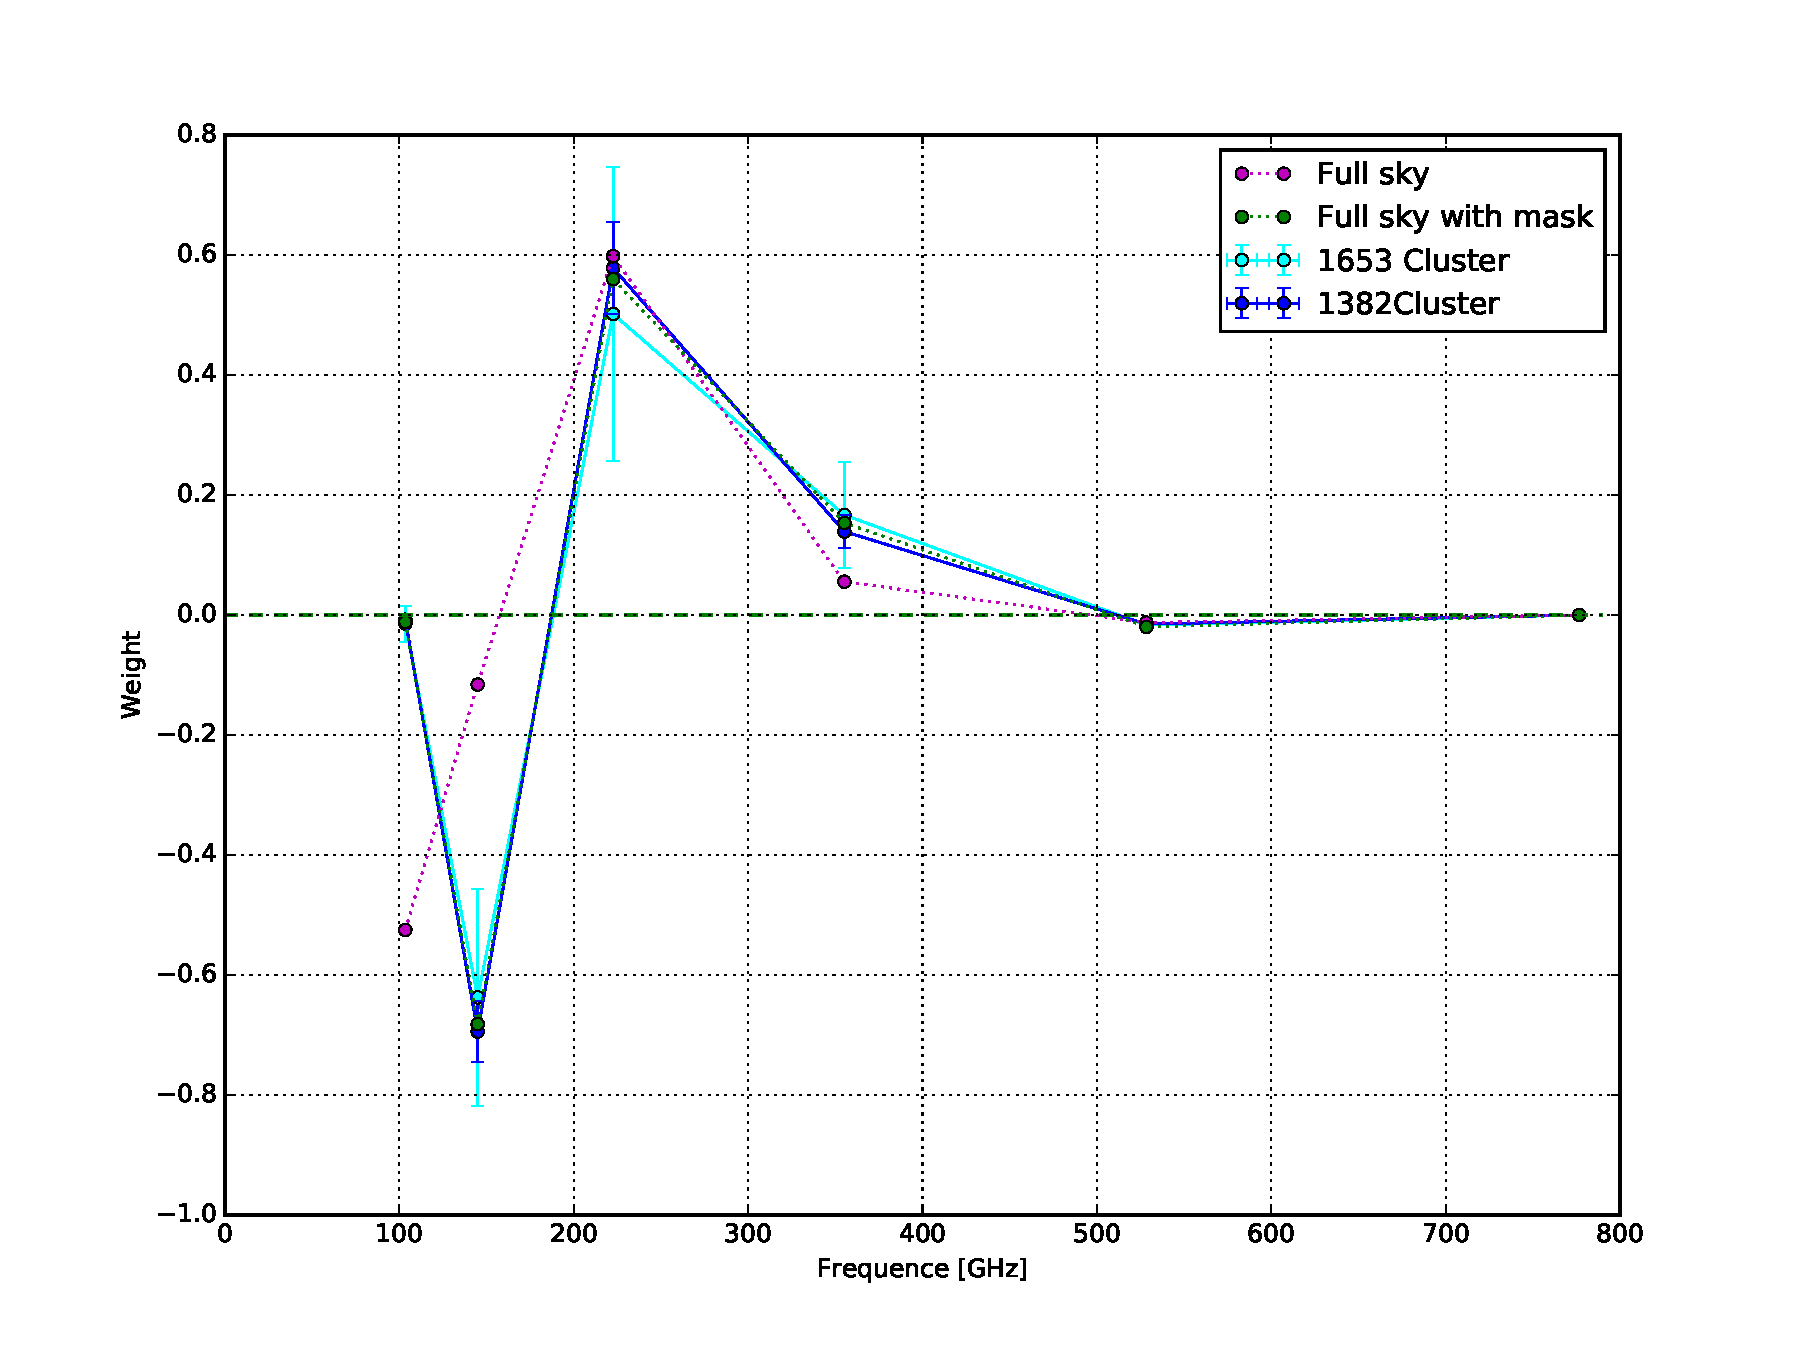
\includegraphics[width=4in]{w_full.pdf}
  \caption{Poids moyen de l'ensemble des amas du catalogue (bleu ciel) et sur
    l'ensemble des amas selectionnés (bleu foncé) en fonction
    de la fréquence. En violet sont réprésentées ces grandeurs pour
    l'ensemble des maps Planck. En vert, l'ensemble des maps avec
    application d'un masque au niveau du plan galactique.}
\end{figure}
  

\section{Photémétrie d'ouverture}
La photometrie d'ouverture est un traitement assez basique qui va nous 
permettre de comparer les flux de nos sources entre eux.
Pour cette procédure nous avons dû définir deux objets : un cercle autour de la source SZ
sur lequel le flux sera calculé et un anneau autour de ce cercle qui va nous servir a estimer le bruit 
aux alentours de la source.

\paragraph{Profil radial des sources.} Les procédures de photometrie s'appuient sur une determination 
du profil radial de nos sources. L'hypothèse de base est que les sources sont circulaires (ce qui n'est 
pas toujours vérifié). La procédure moyenne toutes les valeurs de pixiels equidistants du centre de l'image
pour tracer ce profil radial. Le profil est ensuite normalisé de la facon suivante  : 
\begin{equation}
Pr_n(r) = \frac{Pr(r) - mediane}{\max ( Pr) - mediane}
\end{equation} 
Où $Pr_n(r)$ désigne le profil normalisé et $Pr(r)$ le profil brut et $mediane$ designe une valeur médiane
calculée sur un emsemble de l'image où la source n'apparrait pas (un masque circulaire est posé sur la source).\\

\paragraph{Le cercle.} Pour définir le rayon du cercle, nous avons utilisé la procédure qui nous donne le
profil radial de la source qui nous intéresse. Une fois ce profil normalisé, il est possible de définir un rayon critique
$R_c$ qui va nour permettre de prendre en compte pour chaque source la même proportion du flux total
(similaire à FWMH sur le principe). Concrètement nous avons placé $R_c$ là où le profil radial vaut 40\% du maximum
(cf \ref{profile radial}). \\ 

\paragraph{L'anneau.} Pour des raisons de simplicité le rayon intérieur de l'anneau 
est fixé à $R_{in} = 3R_c $. Si l'on prend un rayon trop grand on risque de prendre en compte dans cet
anneau des amas qui seraient assez proche de notre source.  le rayon externe de l'anneau est fixé à 
$R_{out} = R_{in} + 5  $ (en pixels).

Une fois ces deux objets définis voici la procédure que nous avons suivie pour déterminer le
flux des sources : 
\begin{itemize}
\item On intègre sur le cercle pour obtenir le flux de la source.
\item On intègre sur l'anneau et on divise par la valeur medianne pour estimer le bruit 
aux environs de la source.
\item On soustrait le bruit moyen  au flux de la source.
\end{itemize}
A la fin de cette procédure nous avons donc obtenu des valeurs de flux pour chaque source en 
$\frac{\Delta T}{T}\times pixel $.




\begin{figure}[h!]
  \centering
  \label{profile radial}
  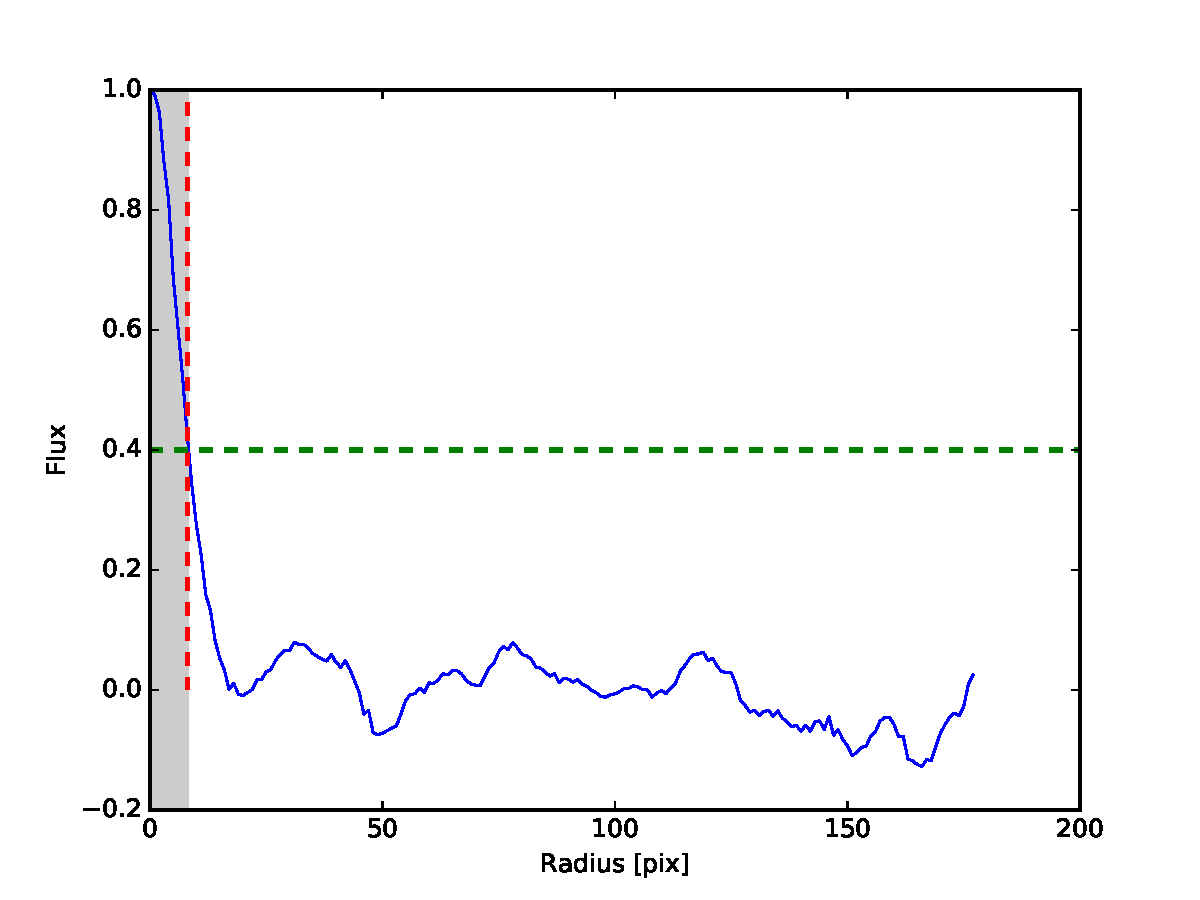
\includegraphics[scale = 0.5]{profile_radiale_ama.pdf}
  \caption{Exemple de profil radial normalisé, tracé pour une source SZ. La Ligne pointillé rouge montre 
  l'emplacement du rayon critique $R_c$ .}
\end{figure}


\begin{figure}[h!]
  \centering
  \label{photometrie d'ouverture}
  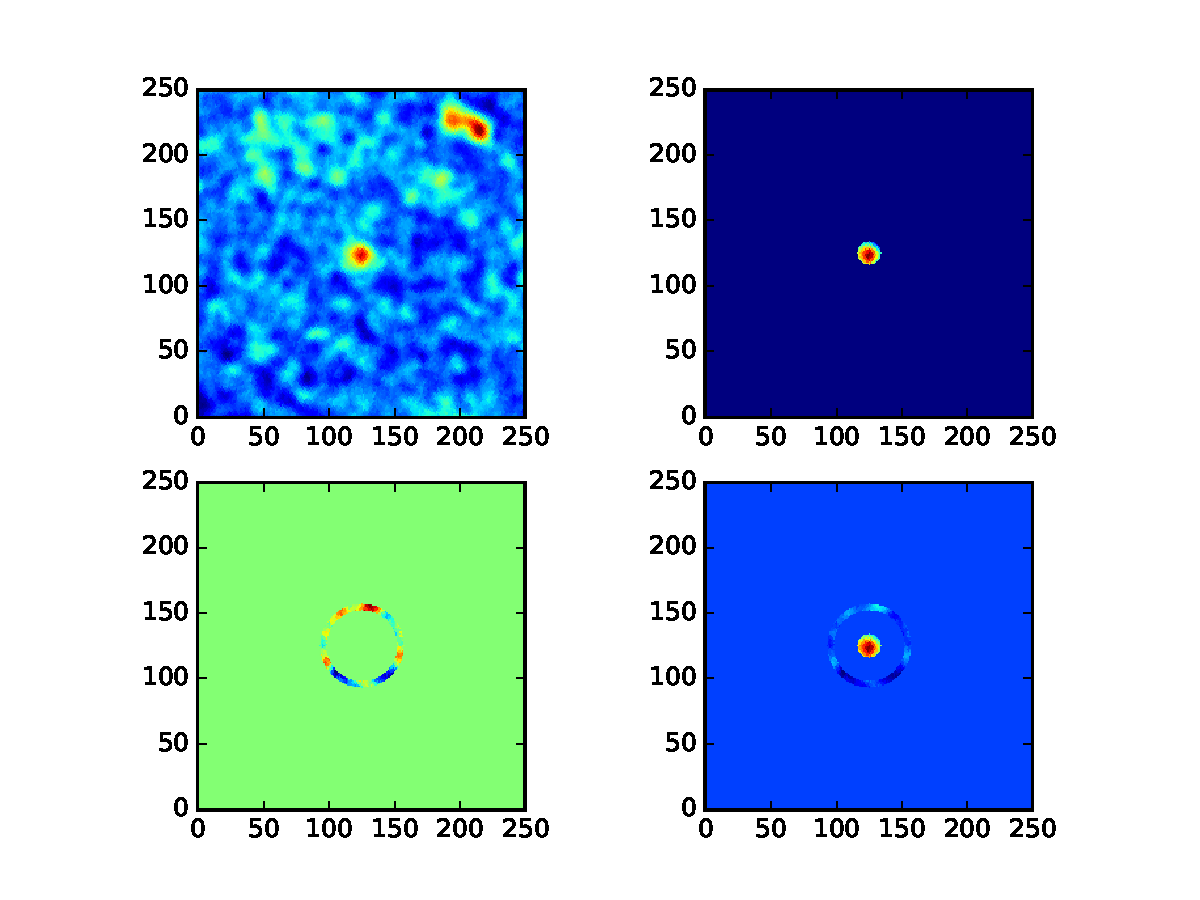
\includegraphics[scale = 0.8]{exemple_photometrie_d'ouverture.pdf}
  \caption{Exemple de cercles et d'anneaux définis pour les procédures de photometrie d'ouverture sur une source SZ. 
  L'anneau et le cercle central sont stockés indépendemment afin de rendre les calculs plus rapides.}
\end{figure}



\paragraph{Discussion sur la methode.} La source majeure d'erreur que nous commettons dans cette procédure provient 
de l'algorithme que nous utilisons pour determiner le rayon critique de nos source. Cependant par manque de temps
 nous avons décidé de ne pas modifier cette méthode. \\
 L'algorithme se contente de prendre le dernier point du profil radial vérifiant : 
 \begin{equation}
 Pr(r) \ge 0.4\times \max (Pr)
 \end{equation}
 Où $Pr$ désigne le profil radial normalisé de la source. 
Comme les valeurs de rayons critiques que nous déterminons ne
peuvent prendre que des valeurs entières, il est plus probable que le rayon critique que nous determinons soit légèrement inférieur au 
rayon qui verifierait exactement : 
\begin{equation}
R = R_c \Leftrightarrow Pr(R_c) = 0.4\times \max (Pr)
\end{equation}
L'erreur que nous commetons ainsi sur la valeur de $r_c$ est de au plus 1 pixel et est asymetrique. Cette erreur 
se répercute evidemment sur le calcul des flux. Nous n'avons malheureusement pas étudié cette répercussion de
façon plus précise.



\section{Résultats et discussion}
Une fois tous les profils de source récupérés, il est possible de determiner un profil typique de source
en fonction de leur rayon critique (cf Fig. \ref{profils_medians}). On peut voir en pointillé une estimation de 
la PSF : profil gaussien avec une largeur à mi-hauteur, déterminée à partir de la carte de Planck 
avec la résolution la moins bonne. On voit sur cette figure que le profil médian correspondant à 
$R_c = 5 $ est en dessous de la PSF. \\
Une explication possible est qu'il y ait un excès de bruit positif à proximité de la source qui nous intéresse.
Cela aurait pour effet de diminuer la valeur du rayon critique de la source et potentiellement faire passer 
le profil en-dessous de la PSF. Le fait que l'on observe sur le graphe une bosse négative semble être en faveur
de cette idée. \\
Pour résoudre ce problème il serait envisageable d'ajuster une gaussienne (avec deux
paramètres : off-set et largeur à mi-hauteur ) sur une section du profil radial que l'on sait n'être
pas contaminé par le bruit (près du centre du profil). Il faut ensuite replacer cette gaussienne de façon à ce que les queues de
la gaussienne soient au niveau de 0 et refaire tourner l'algorithme qui determine le rayon critique
sur ce nouveau profil. On devrait normalement récupérer une valeur plus élevée de $R_c$.

Il serait également intéressant de savoir si la forme des profils obtenus est universelle. En pratique, pour notre
étude, cela consisterait à ramener touts nos profils à un même rayon.

\begin{figure}[h!]
  \centering
  \label{profils_medians}
  \label{radius}
  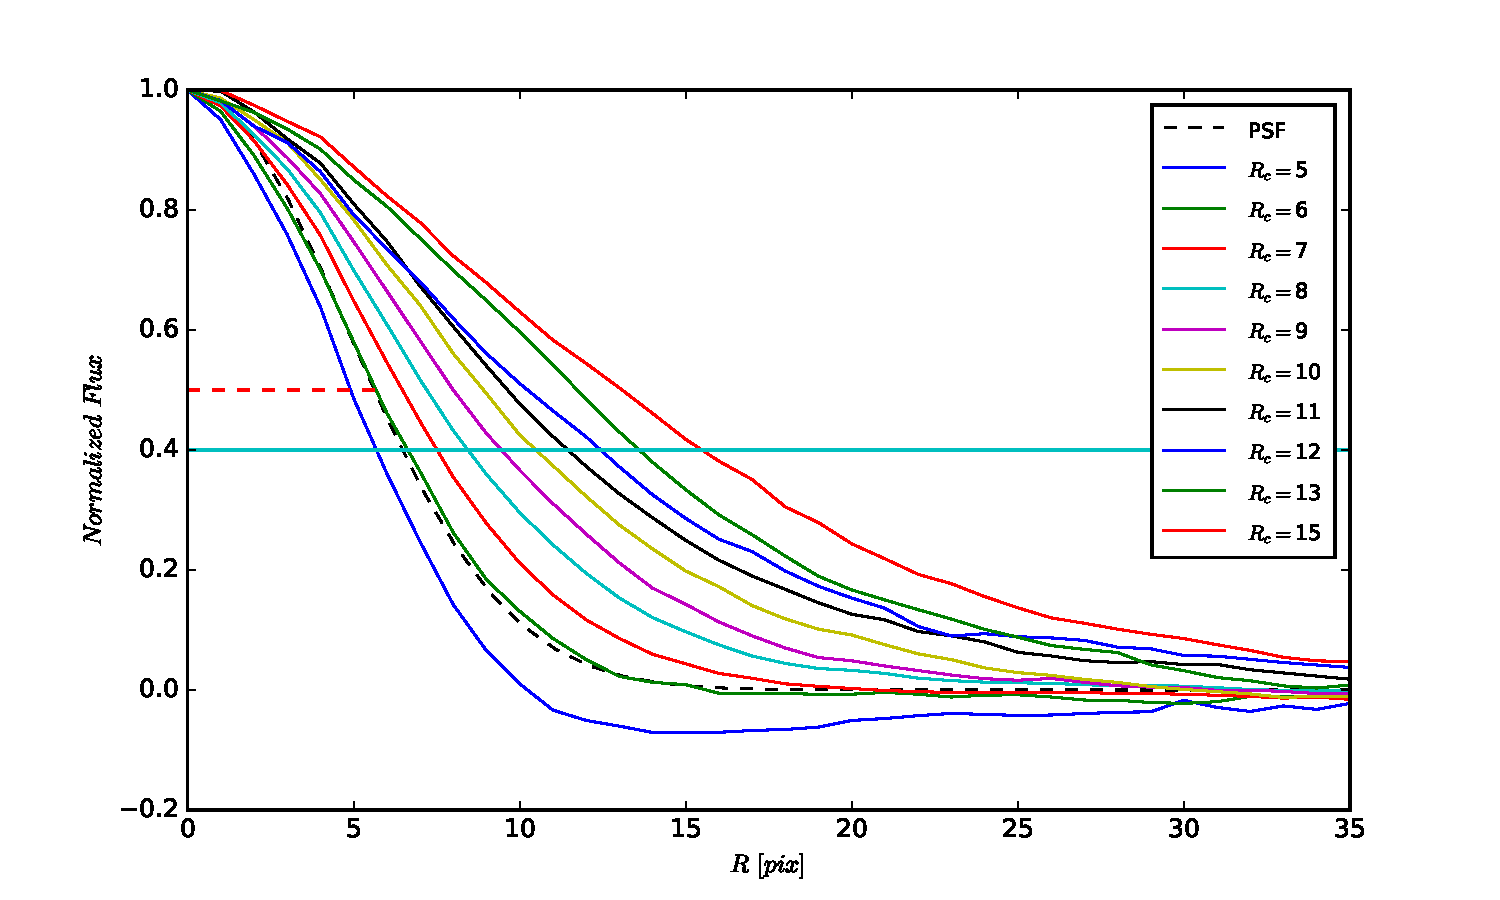
\includegraphics[scale = 0.5]{radius.pdf}
  \caption{Profil typique de sources, médianné sur toutes les sources possédant le même rayon critique}
\end{figure}

\begin{figure}[h!]
  \centering
  \label{rslt_1}
  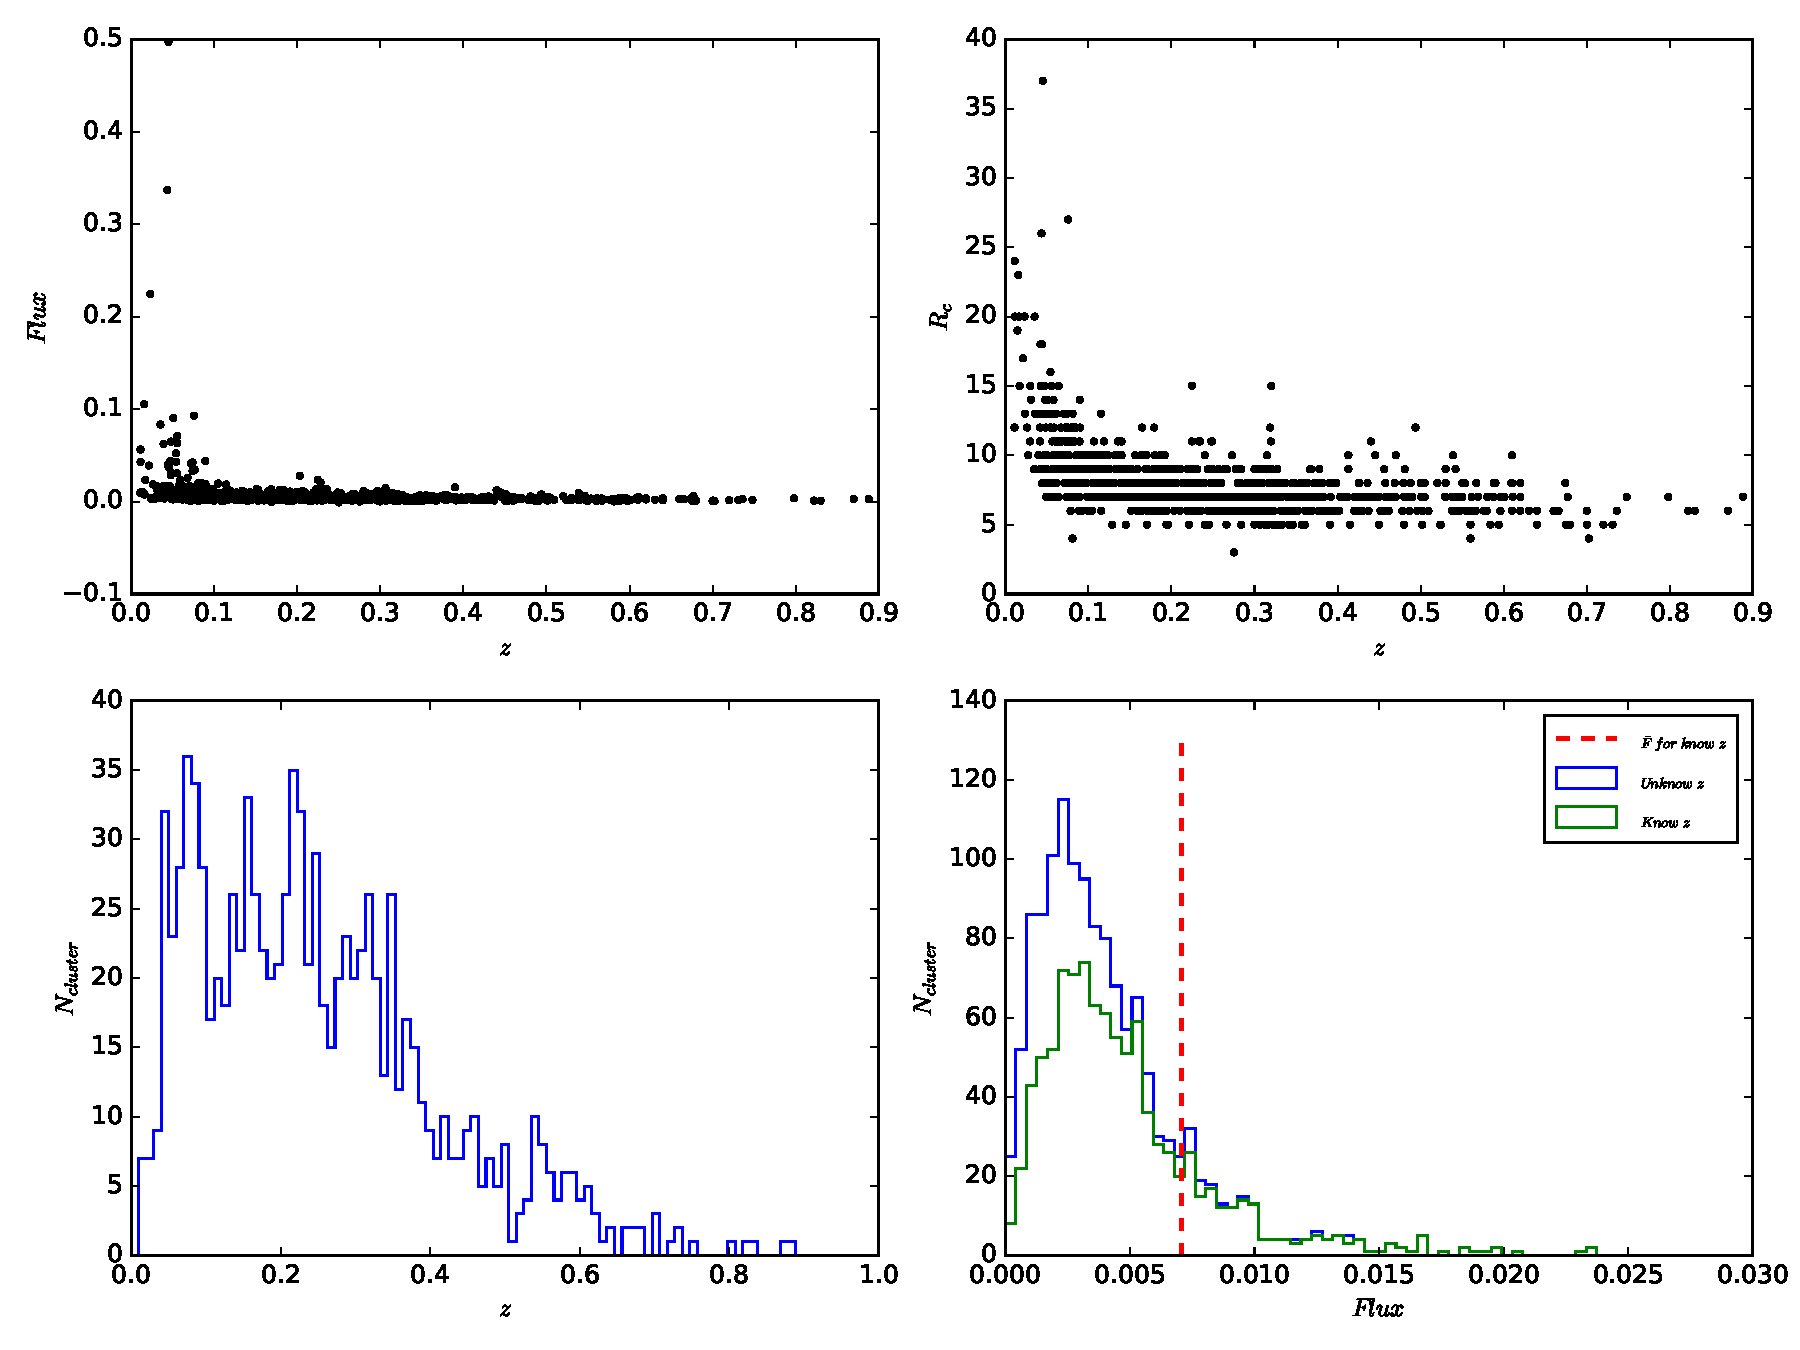
\includegraphics[scale = 0.4]{rslt_1.pdf}
  \caption{En haut à gauche est réprésenté le flux de chaque amas
    selectionné en fonction de son redshift. En haut à droite, le rayon critique
    $R_c$ en fonction du redshift. En bas à gauche l'histogramme des
    redshifts. En bas à droite les histogrammes des flux pour les amas
    dont on connait le redshift (vert) et pour la totalité des amas
    selectionnés au préalable : i.e latitude (bleu).}
\end{figure}

Les résultats de la photométrie d'ouverture effectuée sur les amas
selectionnés au préalable sont présentés Figure
\ref{rslt_1}. L'histogramme des redshifts associés au amas du
catalogue ne montre pas une distribution uniforme. Il y a plus
d'amas détecté à bas redshift qu'à haut redshift. Cela ne devrait
théoriquement pas se produire car pour une masse donnée, le flux SZ
est indépendant du redshift. Ces observations peuvent s'expliquer par
le fait que lorsque le diamètre angulaire de l'amas observé est trop
petit, son effet SZ est totalement dilué par le bim de
l'instrument. On voit donc moins d'amas à haut redshift en raison des
contraintes observationelles de l'instrument Planck. L'évolution de
$R_c$ nous montre en effet une limite qui semble être atteinte pour $5$ pixel,
soit environ $4.3'$. Nous distinguons néanmoins que $R_c$ décroit avec
le redshift, ce qui semble réaliste avec le modèle hiérarchique de
formation des structures. \\

La suite logique de cette étude serait de comparer, en prenant en
compte que le comptage est biaisé, le nombre d'amas par intervals de
redshifts  et par intervals de signal sur bruit pour contraindre le modèle
théorique actuel de formation des grandes stuctures et plus
directement certains paramètres cosmologiques. C'est ce que la
collaboration Planck a étudié dans son dernier article sur le sujet. (voir Planck 2015
results. XXIV \cite{Planck_SZ}) 

\newpage
\begin{thebibliography}{2}
  \addcontentsline{toc}{chapter}{Bibliographie} 

\bibitem{Sunyaev} Sunyaev, R. A., \& Zeldovich, Y. B. 1972, Comments on
  Astrophysics and Space Physics, 4, 173 \\
  
\bibitem{Remazeilles}Remazeilles M. \& al., CMB and SZ effect
  separation with Constrained Internal Linear Combinations, 
  Mon. Not. R. Astron. Soc. 410, 2481–2487 (2011)  \\

\bibitem{Planck_SZ} Planck 2015 results. XXIV. Cosmology from Sunyaev-Zeldovich
cluster counts, Astronomy \& Astrophysics manuscript no. szcosmo 2014
\end{thebibliography}

%\listoffixmes
\end{document}
